\scanpage{15}
\begingroup
\makeatletter
\tagsleft@true
\makeatother
\uline{\deleted{\unsure{I|V}}Version I}

Soient $X$ un espace topologique, $(\deleted{\unsure{\Sigma|S}}E_i)_{i\in I}$ un ens. de % GUIDE01: full-scan origin (190,169), local coordinates in source pixels.
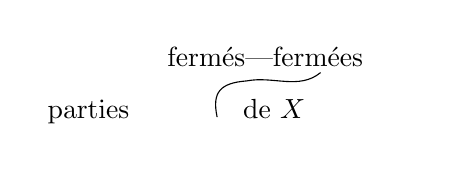
\begin{tikzpicture}[x=.013cm,y=-.013cm,baseline=(p.base),line cap=round,line join=round]
\path[use as bounding box] (0,0) rectangle (385,113);
\node[anchor=base west,inner sep=0pt] (p) at (19,89) {parties};
\node[anchor=base west,inner sep=0pt] at (210,89) {de $X$};
\node[anchor=base west,inner sep=0pt] at (136,38) {\inserted{\unsure{fermés|fermées}}};
\draw (185,87) .. controls (180,63) and (188,54) .. (214,52)
 .. controls (240,47) and (265,61) .. (286,44);
\end{tikzpicture} (noté indiciellement), telles que l'on ait
% slanted
\reversemarginpar
\margin{$\nearrow$ On suppose de plus que pour \unsure{tte|toute|tt} comp. conn. $\unsure{\Sigma_i|\Sigma}$ de $X\setminus E_i$, on ait $\overline{\Sigma}_i\cap E_i\ne\varnothing$ i.e. $\overline{\Sigma}_i\ne\Sigma_i$ i.e. $\Sigma_i$ non fermé dans $X$ (ce qui est le cas si $X$ est connexe)}
\normalmarginpar
\[
 \forall i\in I,\quad \operatorname{Card}\pi_0(X\setminus\deleted{\Sigma}E_i)=2
 \tag*{(a)}
\]
\margin{\uline{NB} les comp. conn. $\Sigma_i^+,\Sigma_i^{\unsure{+|-|\ast}}$ de $X\setminus\Sigma_i$ sont ouvertes dans $X$}
\[
 \begin{aligned}
 &\forall(i,j)\in I\times I,\ i\ne j,\quad \deleted{\Sigma}E_j\ \text{est contenu dans l'une}\\
 &\text{des deux composantes connexes de }X\setminus\deleted{\Sigma}E_i.
 \end{aligned}
 \tag*{(b)}
\]

NB Cette condition (b) est vérifiée automatiquement les $\deleted{\Sigma}E_i$ $(i\in I)$ sont connexes, dès lors que les $E_i$ sont supposés disjoints mutuellement

On se propose d'étudier le ``découpage'' de $X$ par la famille $(E_i)$.

% RULE01/RULE02: full-scan origin (500,994); the underline has two visible runs.
\figure{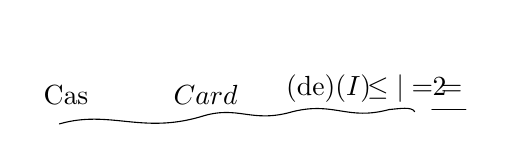
\begin{tikzpicture}[x=.013cm,y=-.013cm,line cap=round,line join=round]
\path[use as bounding box] (0,0) rectangle (458,106);
\node[anchor=base west,inner sep=0pt] at (15,75) {Cas};
\node[anchor=base west,inner sep=0pt] at (142,75) {$\operatorname{Card}$};
\node[anchor=base west,inner sep=0pt] at (252,66) {$\deleted{\unsure{(\mathrm{de})}}(I)$};
\node[anchor=base west,inner sep=0pt] at (331,66) {$\deleted{\unsure{\leq|=}}=$};
\node[anchor=base west,inner sep=0pt] at (395,66) {$2$};
\draw (31,94) .. controls (80,80) and (111,104) .. (169,87)
 .. controls (206,75) and (218,94) .. (259,82)
 .. controls (300,72) and (312,91) .. (353,80)
 .. controls (364,79) and (375,77) .. (378,82);
\draw (395,80) -- (428,80);
\end{tikzpicture}}

Soit $\Sigma_i^+$ la comp. conn. de $X\setminus E_i$ qui ne contient pas $E_j$ $(j\ne i)$, alors on a (si $I=\{1,2\}$)
% DRAW01: full-scan origin (19,1038), fixed local source-pixel rectangle.
% C's two left-brace paths and right-brace path are retained after checking,
% with local translation (5,33), i.e. full-scan origin (24,1071) for those paths.
\figure{\begin{tikzpicture}[x=.013cm,y=-.013cm,line cap=round,line join=round]
\path[use as bounding box] (0,0) rectangle (553,336);
% Oval: visible strong runs, pale runs and short gaps are distinct paths.
\draw (186,122) .. controls (210,76) and (262,35) .. (290,38)
 .. controls (342,35) and (380,88) .. (402,160);
\draw (403,168) .. controls (405,185) and (403,206) .. (401,216);
\draw[black!45] (401,217) .. controls (401,226) and (398,235) .. (394,243);
\draw (391,249) .. controls (387,257) and (382,263) .. (378,267);
\draw (374,273) .. controls (369,282) and (365,287) .. (361,291);
\draw (358,295) .. controls (334,319) and (294,320) .. (269,315)
 .. controls (219,309) and (178,276) .. (169,220)
 .. controls (166,206) and (168,197) .. (168,193);
\draw (168,193) .. controls (163,196) and (163,190) .. (166,181);
\draw (168,193) -- (173,185);
\draw[black!45] (168,179) .. controls (174,160) and (179,139) .. (186,122);
% Chords, separately checked at both rim contacts.
\draw[line width=.8pt] (186,122) .. controls (247,125) and (324,109) .. (392,119)
 (176,250) .. controls (242,253) and (328,246) .. (391,239);
\begin{scope}[shift={(5,33)}]
\draw (44,9) .. controls (46,57) and (63,106) .. (32,108)
 .. controls (52,132) and (38,151) .. (46,195) -- (55,228);
\draw (41,109) .. controls (72,143) and (35,144) .. (48,193)
 .. controls (47,224) and (57,241) .. (39,252) .. controls (55,242) and (43,259) .. (49,282);
\draw (428,86) .. controls (439,93) and (409,141) .. (434,149)
 .. controls (420,158) and (436,251) .. (417,254);
\end{scope}
% Cancelled label: one visible text copy, actual crossing paths, invisible deletion annotation.
\node[inner sep=0pt] at (167,48) {\rlap{$\unsure{\Sigma_1^+|\Sigma_2^+}$}\phantom{$\deleted{\unsure{\Sigma_1^+|\Sigma_2^+}}$}};
\draw (138,60) -- (198,27);
\draw (151,42) .. controls (161,20) and (181,12) .. (177,24) -- (149,52);
\node at (139,116) {$E_1$}; \node at (150,247) {$E_2$};
\node at (430,68) {$\Sigma_1^+$};
\node at (501,193) {$\Sigma_1^{\deleted{\unsure{+}}\unsure{-}}$};
\node at (23,135) {$\Sigma_2^-$}; \node at (131,308) {$\Sigma_2^+$};
% MARK01: detached short dot above the right overwritten superscript;
% full-scan observed bbox approximately (525,1189,531,1198), role/hand unresolved.
\node[inner sep=0pt] at (509,156) {\unsure{\begin{tikzpicture}[x=.013cm,y=-.013cm]
\path[use as bounding box] (0,0) rectangle (4,6);
\fill (1,0) .. controls (4,1) and (4,4) .. (2,6) .. controls (0,5) and (0,2) .. (1,0);
\end{tikzpicture}}};
\end{tikzpicture}}

\[
 \Sigma_1^+\cap\Sigma_2^+=\varnothing
 \tag*{(1)}
\]
ce qui \deleted{résulte de}
\[
 \begin{aligned}
 &\deleted{\Sigma_1^-\supset\Sigma_2^+}\qquad\text{\unsure{équivaut|èquivaut} à}\\
 &\deleted{\Sigma_2^-\supset\Sigma_1^+}\qquad \Sigma_1^+\subset\Sigma_2^-\cup E_2,\quad\text{et}
 \end{aligned}
\]
% CANCEL01/CANCEL02: full-scan origin (206,1437); two cancellation runs.
\figure{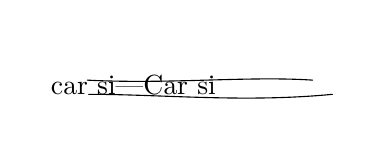
\begin{tikzpicture}[x=.018cm,y=-.018cm,line cap=round]
\path[use as bounding box] (0,0) rectangle (232,73);
\node[anchor=base west,inner sep=0pt] at (16,47) {\rlap{\unsure{car si|Car si}}\phantom{\deleted{\unsure{car si|Car si}}}};
\draw (42,37) .. controls (100,40) and (155,34) .. (201,37);
\draw (43,47) .. controls (95,47) and (153,53) .. (215,47);
\end{tikzpicture}}
\deleted{Si on avait} comme $\Sigma_1^+\cap E_2=\varnothing$, cela équivaut aussi à
\[
 \Sigma_1^+\subset\Sigma_2^-
 \tag*{(2)}
\]
\unsure{et} \unsure{symètriquement|symétriquement}, à
\[
 \Sigma_2^+\subset\Sigma_1^-
 \tag*{$(2')$}
\]

Comme
% MARK02 and raised cancelled words: full-scan origin (409,2008).
\begin{tikzpicture}[x=.013cm,y=-.013cm,baseline=(inc.base),line cap=round]
\path[use as bounding box] (0,0) rectangle (319,136);
\node[anchor=base west,inner sep=0pt] at (16,42) {\deleted{\unsure{vois. ouvert}}};
\node[anchor=base west,inner sep=0pt] (inc) at (75,113) {$\Sigma_2^-\supset E_1$,};
\node[inner sep=0pt] at (111,61) {\unsure{\begin{tikzpicture}[x=.013cm,y=-.013cm,line cap=round]
\path[use as bounding box] (0,0) rectangle (19,16);
\draw[line width=.6pt] (1,15) .. controls (8,7) and (13,3) .. (18,2);
\end{tikzpicture}}};
\end{tikzpicture} \deleted{il contient les} \inserted{i.e. $\Sigma_2^-$ est un \uline{vois.} ouvert de $E_1$,} on a
% slanted
\reversemarginpar
\margin{$\overline{\Sigma_1^+}\cap E_1\ne\varnothing$ i.e. $\overline{\Sigma_1^+}\ne\Sigma_1^+$ \unsure{à sign.ler|à signaler} avant}
\normalmarginpar
% GUIDE02: observed curved stroke above the first Sigma of the next display.
% Fixed full-scan origin (180,2158); no character or mathematical role assigned.
\figure{\begin{tikzpicture}[x=.013cm,y=-.013cm,line cap=round]
\path[use as bounding box] (0,0) rectangle (125,67);
\node[inner sep=0pt] at (62,33) {\unsure{\begin{tikzpicture}[x=.013cm,y=-.013cm,line cap=round]
\path[use as bounding box] (0,0) rectangle (125,67);
\draw[black!65] (7,59) .. controls (0,34) and (22,28) .. (60,21)
 .. controls (87,18) and (105,13) .. (118,7);
\end{tikzpicture}}};
\end{tikzpicture}}
\[
 \Sigma_2^-\cap\Sigma_1^+\ne\varnothing
\]
Car $\underline{\overline{\Sigma_1^+}\cap E_1}\ne\varnothing$ % GUIDE03: full-scan origin (1274,2097); hooked insertion guide retained.
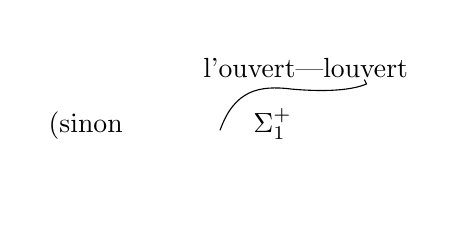
\begin{tikzpicture}[x=.013cm,y=-.013cm,baseline=(sin.base),line cap=round,line join=round]
\path[use as bounding box] (0,0) rectangle (386,173);
\node[anchor=base west,inner sep=0pt] (sin) at (20,102) {(sinon};
\node[anchor=base west,inner sep=0pt] at (220,102) {$\Sigma_1^+$};
\node[anchor=base west,inner sep=0pt] at (171,49) {\inserted{\unsure{l'ouvert|louvert}}};
\draw (188,100) .. controls (202,61) and (226,56) .. (258,60)
 .. controls (292,63) and (317,61) .. (331,55) -- (329,51);
\end{tikzpicture} serait \inserted{un} fermé dans $X$, \unsure{donc|puis} % CANCEL03: full-scan origin (920,2238), one text copy and visible overstrikes.
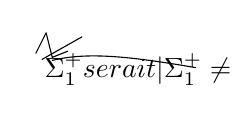
\begin{tikzpicture}[x=.013cm,y=-.013cm,baseline=(del.base),line cap=round,line join=round]
\path[use as bounding box] (0,0) rectangle (177,67);
\node[anchor=base west,inner sep=0pt] (del) at (16,49) {\rlap{$\unsure{\Sigma_1^+\text{ serait}|\Sigma_1^+\ne\varnothing}$}\phantom{$\deleted{\unsure{\Sigma_1^+\text{ serait}|\Sigma_1^+\ne\varnothing}}$}};
\draw (14,31) -- (53,9);
\draw (8,25) -- (18,5) -- (24,29) -- (39,23);
\draw (24,32) .. controls (60,23) and (105,29) .. (164,39);
\end{tikzpicture} $X$ serait disconnexe),
\endgroup
% archive sheet number: 14
